\section{Khu vực nghiên cứu}

Đồ án tập trung vào toàn bộ vùng quy hoạch lâm nghiệp của tỉnh Cà Mau mới (đã giới thiệu tại Mục 1.1.3). Dữ liệu ranh giới quy hoạch lâm nghiệp được cung cấp bởi Công ty TNHH Tư vấn và Phát triển Đồng Xanh — đối tác của Chi cục Kiểm lâm tỉnh Cà Mau.

\begin{figure}[H]
    \centering
    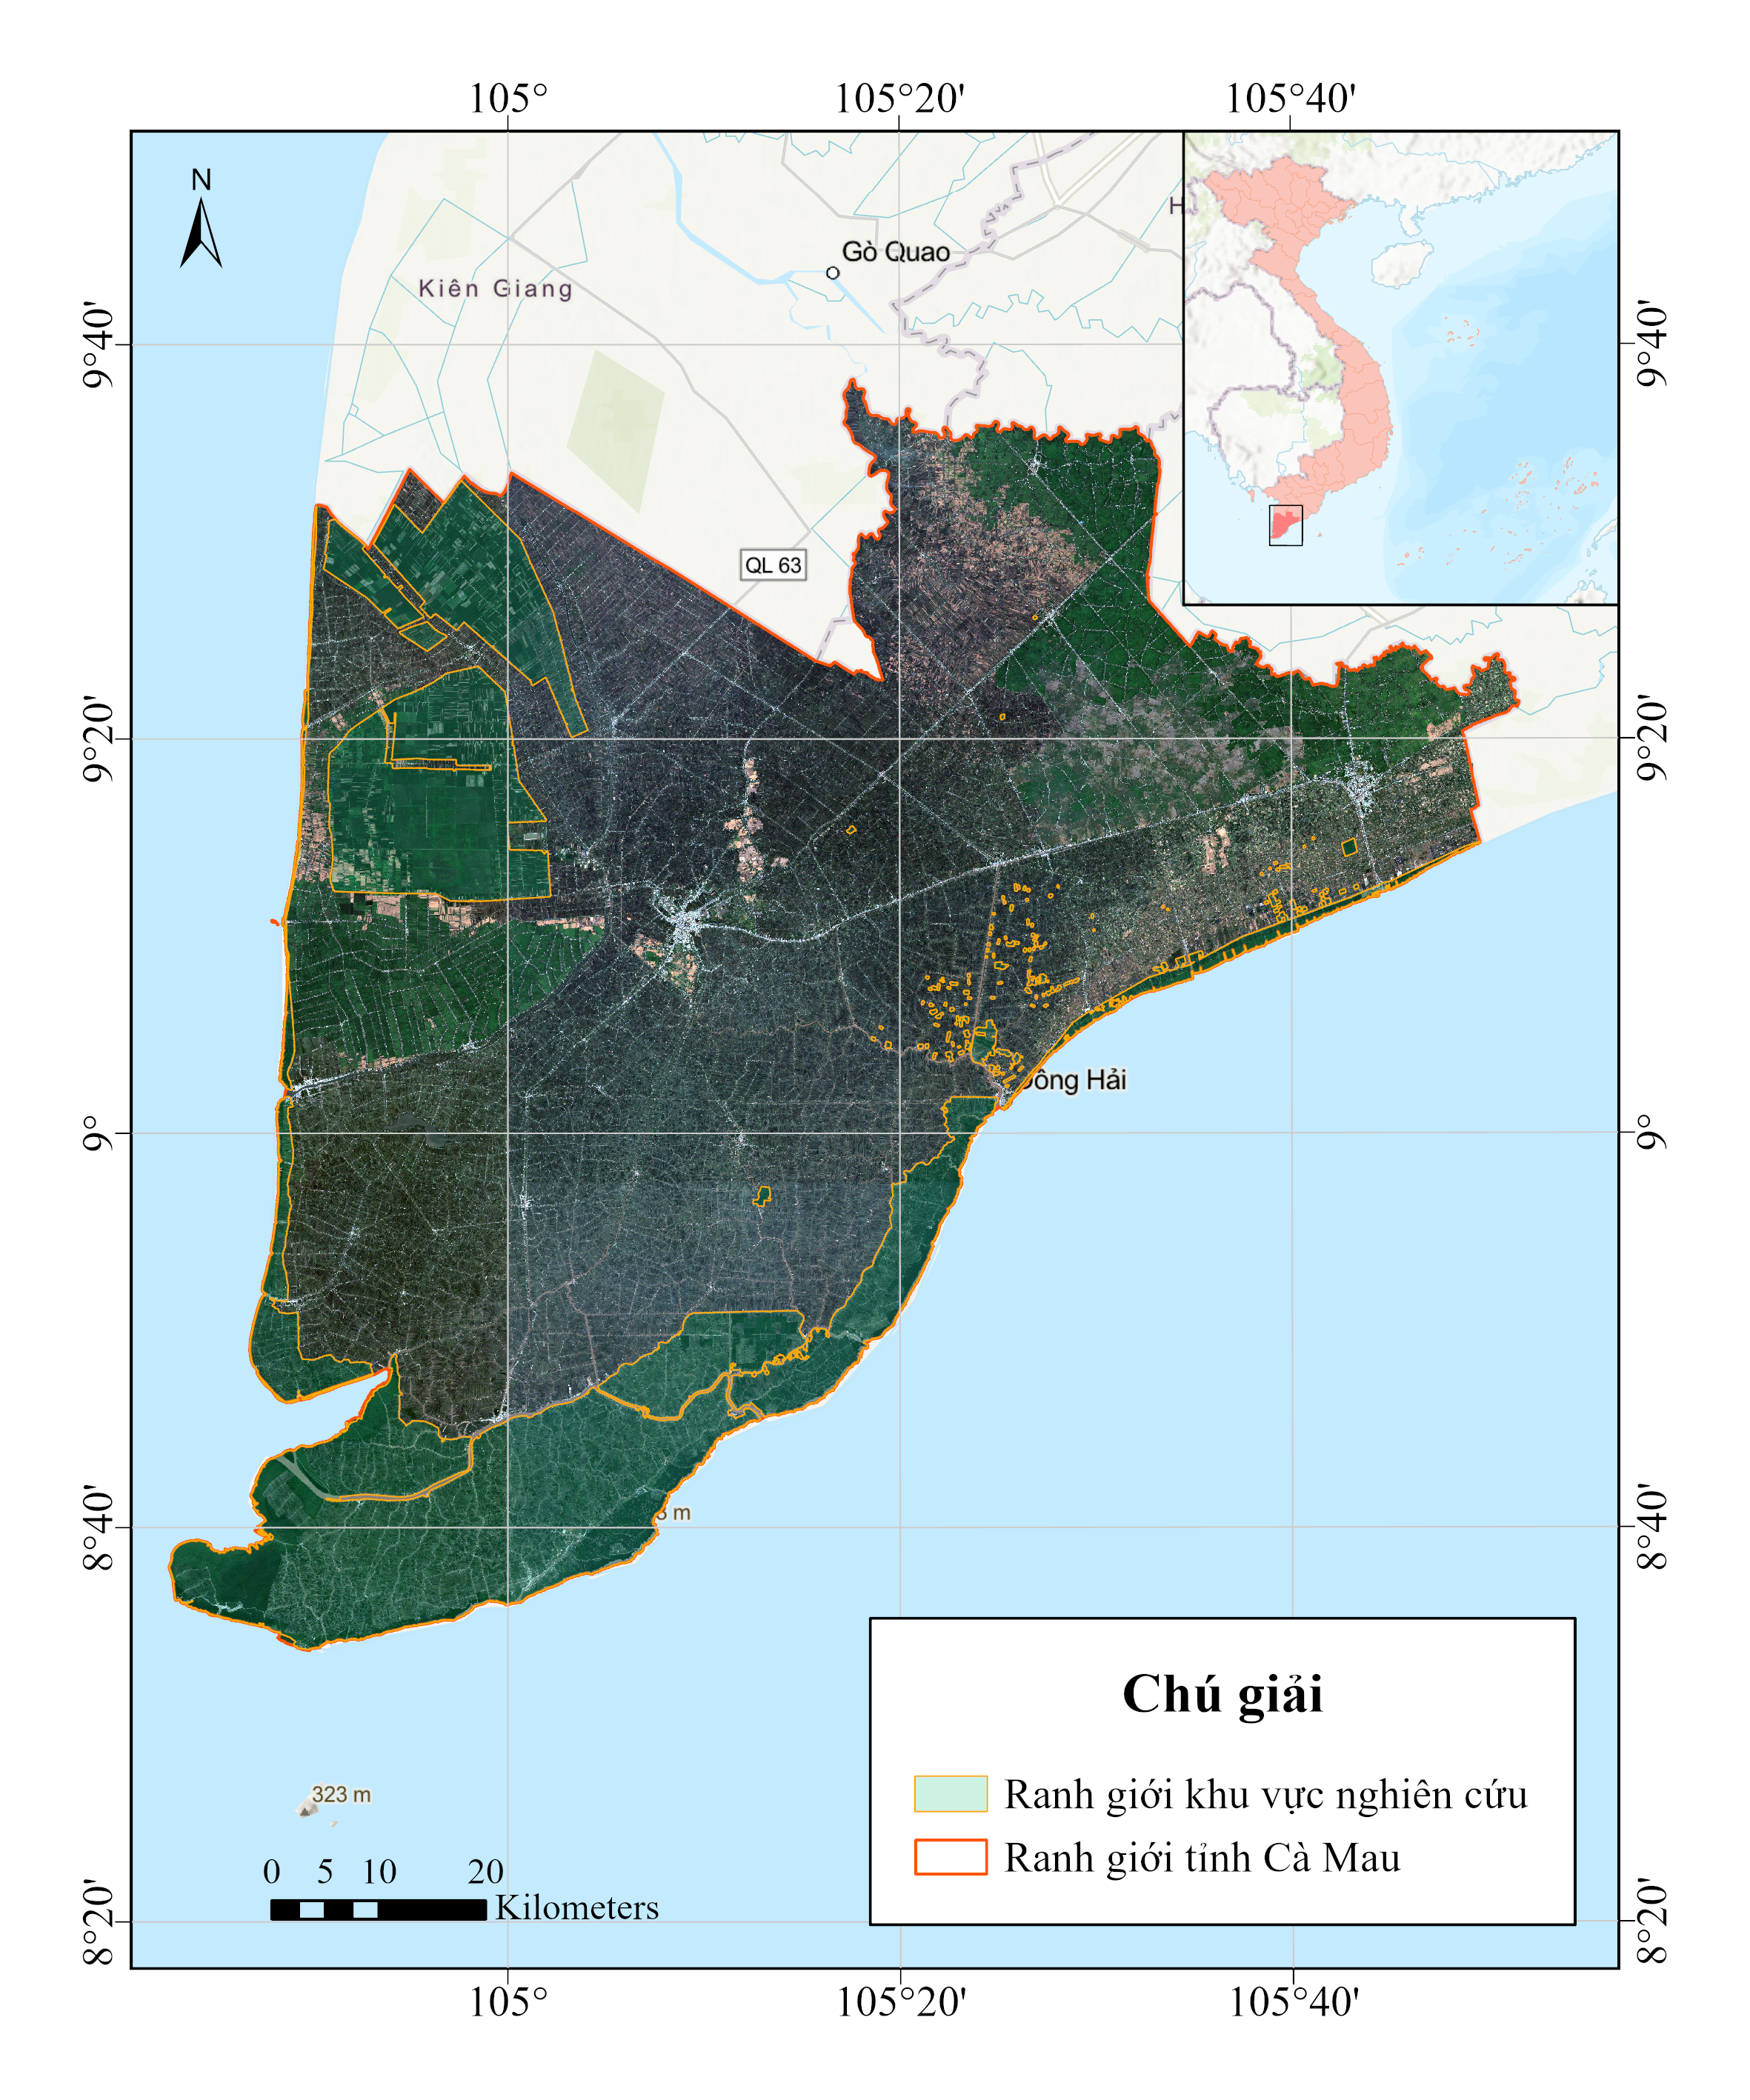
\includegraphics[width=0.95\textwidth]{img/chapter1/RGB-Ca-Mau.png}
    \caption{Ảnh vệ tinh tổ hợp màu tự nhiên (RGB) khu vực nghiên cứu tỉnh Cà Mau.}
    \label{fig:study_area}
\end{figure}

Tổng diện tích ranh giới quy hoạch là 170,178.82 hecta (tương đương 1,701.79 km²), bao gồm 666 polygon trong file shapefile ranh giới. Diện tích thực tế được phân loại là 162,468.50 hecta (khoảng 95.5\% diện tích ranh giới); phần còn lại (~7,710 ha, chiếm 4.5\%) bị loại do mây che phủ hoặc dữ liệu không hợp lệ (nodata) trong quá trình xử lý ảnh vệ tinh. Kích thước raster là 12,547 × 10,917 pixels (ở độ phân giải 10m), sử dụng hệ quy chiếu EPSG:32648 (WGS 84 / UTM Zone 48N).
